\documentclass[twocolumn,prd,aps,superscriptaddress,preprintnumbers,tightenlines,showpacs,nofootinbib,eqsecnum,amsfonts,amsmath]{revtex4-1}
\usepackage{epsfig}
\usepackage{graphics}
\usepackage{graphicx}
\usepackage{bm}
\usepackage[dvipsnames]{xcolor}
\usepackage{bm}
\usepackage{times}
\usepackage{xspace}
\usepackage[varg]{txfonts}
\usepackage[normalem]{ulem} % To get strikethrough (\sout)
\usepackage[colorlinks]{hyperref}
\usepackage[caption=false]{subfig}
\usepackage{booktabs}
\usepackage{url}
\usepackage{float}
\usepackage[bottom]{footmisc}
\usepackage{lineno}
\usepackage{makecell}

\definecolor{LinkColor}{rgb}{0.75, 0, 0}
\definecolor{CiteColor}{rgb}{0, 0.5, 0.5}
\definecolor{UrlColor}{rgb}{0, 0, 0.75}
\hypersetup{linkcolor=LinkColor}
\hypersetup{citecolor=CiteColor}
\hypersetup{urlcolor=UrlColor}
\usepackage{perpage}
\MakePerPage{footnote}

\newcommand{\paperone}{Paper~I\xspace}
\newcommand{\abhi}[1]{\textcolor{Emerald}{[AG: #1]}}
\newcommand{\rb}[1]{\textcolor{blue}{[\textit{RB: #1}]}}
\newcommand{\ab}[1]{\textcolor{cyan}{#1}}
\newcommand{\comment}[1]{\textcolor{red}{[#1]}}
\newcommand{\macro}[1]{\textcolor{orange}{\textbf{#1}}}

\newcommand{\h}{\mathpzc{h}}
\newcommand{\Hhat}{\hat{\mathpzc{H}}}
\newcommand{\B}{\mathpzc{B}}
\newcommand{\hlm}{\mathpzc{h}_{\ell m}}
\newcommand{\xilm}{\xi_{\ell m}}
\newcommand{\Ylm}{{Y}^{-2}_{\ell m}}
\newcommand{\Y}{{Y}^{-2}}
\newcommand{\hc}{h_\times}
\newcommand{\hp}{h_+}
\newcommand{\Fc}{F_\times}
\newcommand{\Fp}{F_+}
\newcommand{\Mf}{M_f}
\newcommand{\cA}{\mathpzc{A}}
\newcommand{\lm}{_{\ell m}}
\newcommand{\deff}{d_\mathrm{eff}}
\newcommand{\rmi}{\mathrm{i}}
\newcommand{\blambda}{\bm{\lambda}}
\newcommand{\btheta}{\bm{\theta}}
\newcommand{\bxi}{\bm{\xi}}
\newcommand{\bxigr}{\bm{\xi}_{\text{GR}}}
\newcommand{\bxingr}{\bm{\xi}_{\text{nGR}}}
\newcommand{\bzeta}{\bm{\zeta}}
\newcommand{\bs}[1]{\bm{\vec{S}_{#1}}}
\newcommand{\Mo}{M_{\odot}}
\newcommand{\FFe}{\mathrm{FF}_\mathrm{eff}}
\newcommand{\FF}{\mathrm{FF}}
\newcommand{\e}{\mathrm{e}}
\newcommand{\rhoopt}{\rho_\mathrm{opt}}
\newcommand{\rhosubopt}{\rho_\mathrm{subopt}}
\newcommand{\fqnm}{f}
\newcommand{\sigmaqnm}{\sigma}
\newcommand{\n}{\mathbf{n}}
\newcommand*{\skymapscale}{0.5}
\newcommand*{\paramestscale}{0.455}
\newcommand{\df}[1]{\delta f_{\text{#1}}}
\newcommand{\dtau}[1]{\delta \tau_{\text{#1}}}
\newcommand{\fngr}[1]{f_{\text{#1}}}
\newcommand{\taungr}[1]{\tau_{\text{#1}}}
\newcommand{\fgr}[1]{f ^{\text{GR}}_{\text{#1}}}
\newcommand{\taugr}[1]{\tau ^{\text{GR}}_{\text{#1}}}
\newcommand{\pSEOB}{\texttt{pSEOBNR}}
\newcommand{\SEOB}{\texttt{SEOBNR}}

\begin{document}

%%%%%%%%%%%%%%%%%
\section{TGR: The \textsc{pSEOBNRv4HM} analysis}
\label{sec:pa_tgr}
Optimisations in waveform generation presented in this paper not only benefit gravitational wave detection and parameter estimation, but would also speed up downstream inferences in astrophysics, cosmology and fundamental physics. We demonstrate this expedition on one of the ringdown tests of general relativity previously discussed in ~\cite{Ghosh:2016xx:prep,Abbott:2020jks,Brito:2018rfr}. The $\pSEOB$ ringdown analysis uses a parameterised version of a full inspiral-merger-ringdown gravitational wave signal model to measure and constrain the (complex) QNM frequencies. Consequently, unlike other ringdown studies restricted to the post-merger signal, the $\pSEOB$ analysis makes use of the entire signal power and does not suffer from the ambiguity of a ringdown start-time definition. However, the current implementation of the test uses the time-domain \texttt{SEOBNRv4HM}~\cite{Cotesta:2018fcv} waveform model and is computationally expensive, especially since every iteration of the parameter estimation sampler requires the generation of a complete inspiral-merger-ringdown waveform. This also makes the $\pSEOB$ analysis an ideal candidate for testing post-adaibatic optimisations.
\par
In the \texttt{SEOBNRv4HM} model, starting from estimates of the initial binary's masses and spins, numerical relativity fits~\cite{Taracchini:2013rva,Hofmann:2016yih} are used to predict the mass and spin of the remnant object, which are then used to predict the ringdown frequencies and damping times, $(f_{\ell m 0}^{\text{GR}}, \tau _{\ell m 0}^{\text{GR}})$~\cite{Berti:2005ys,Berti:2009kk}. In the parameteretised model, (\texttt{pSEOBNRv4HM}), the frequency and damping times, $(f_{\ell m 0}, \tau _{\ell m 0})$ are described through fractional deviations, $(\delta
\hat{f}_{\ell m 0},\delta \hat{\tau}_{\ell m 0})$, from the corresponding GR predictions as:
\begin{eqnarray}
f_{\ell m 0} &=& f_{\ell m 0}^{\text{GR}}\, (1 + \delta \hat{f}_{\ell m 0})\,,\label{eq:nongr_freqs_a} \\ 
\tau _{\ell m 0} &=& \tau _{\ell m 0}^{\text{GR}}\, (1 + \delta \hat{\tau}_{\ell m 0})\,. \label{eq:nongr_freqs_b}
\end{eqnarray}
and left as free parameters in the model, to be directly estimated from the data instead of being predicted using NR fits. A comparison of the measurements of the frequency and damping time for the least-damped QNM for GW150914, $(f_{220},\tau_{220})$, using a version of \texttt{pSEOBNRv4HM} with ("PA") and without ("non-PA") post-adaibatic optimisations is shown in the left panel of Fig.~\ref{fig:pa_nonpa_tgr}. The \texttt{pSEOBNRv4HM} waveform model contains information from $(l,m)=(2,2), (2,1),(3,3), (4,,4)$ and $(5,5)$ modes. For a quasi-equal high-mass binary like GW150914, contributions from higher multipoles of the GW signal are expected to be negligible. Hence, we restrict our analysis to just the least-damped dominant QNM, i.e., $(f_{220},\tau_{220})$, keeping the other QNMs fixed at their nominal GR values. We find that the model with post-adiabatic optimisations faithfully reproduces results without them. However, as shown in the right panel of Fig.~\ref{fig:pa_nonpa_tgr}, the speed-up is significant. Fitting a straight line through the points in the period between when each run started accumulating samples and/or was terminated, the slope of the PA run is roughly 8 times steeper than the non-PA run. In other words, the PA run accumulated samples at a rate 8 times faster than then non-PA run.
\par
With focus shifting from analyses of individual events to population studies, demands on computational resources and person-power are ever-increasing, as demonstrated by large-scale studies in LVK catalog papers CITE(PE/astro-imp/TGR catalog papers). Hence, such increases in computational efficiency is immensely important for the future of GW data analysis.

% Figure for pSEOBNR
\begin{figure*}
  \centering
  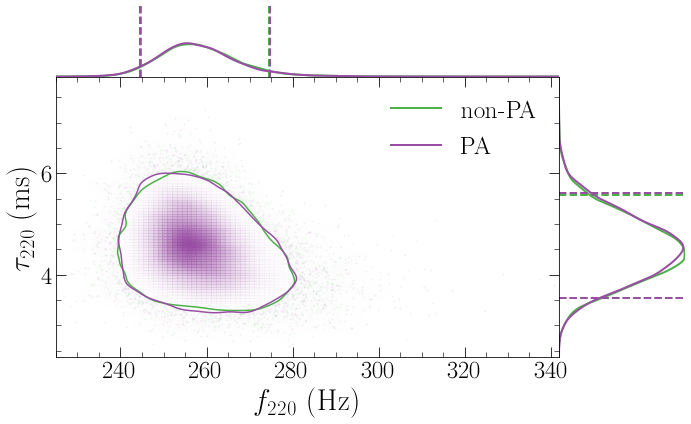
\includegraphics[height=5cm]{GW150914_actual_PA_nonPA_fngrtaungr}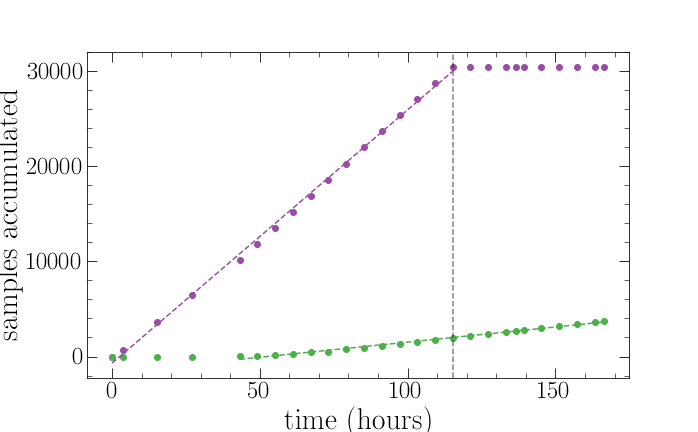
\includegraphics[height=5cm]{GW150914_actual_PA_nonPA_benchmarking}
  \caption{\emph{Left panel}:The 90\% credible levels of the posterior probability distribution of the frequency and damping time of the $(2,\pm 2)$ QNM, $(f_{220},\tau_{220})$ and their corresponding one-dimensional marginalized posterior distributions, for GW150914. \emph{Right panel}: Accumulation of samples over time, usng the PA and non-PA models. The black vertical dashed line indicates the point at which the PA run was terminated. The magenta (green) dashed line represents a straight line fitted to the PA (non-PA) points, restricted to the period over which the run accummulated samples. The PA run accumulated samples roughly 8 times faster than the non-PA run.}
  \label{fig:pa_nonpa_tgr}
\end{figure*}

%%%%%%%%%%%%%%%%%

%%%%%%%%%%%%%%%%%
\bibliographystyle{apsrev}
\bibliography{pa_tgr_section}
%%%%%%%%%%%%%%%%%

\end{document}
